% Training Pipeline Diagram
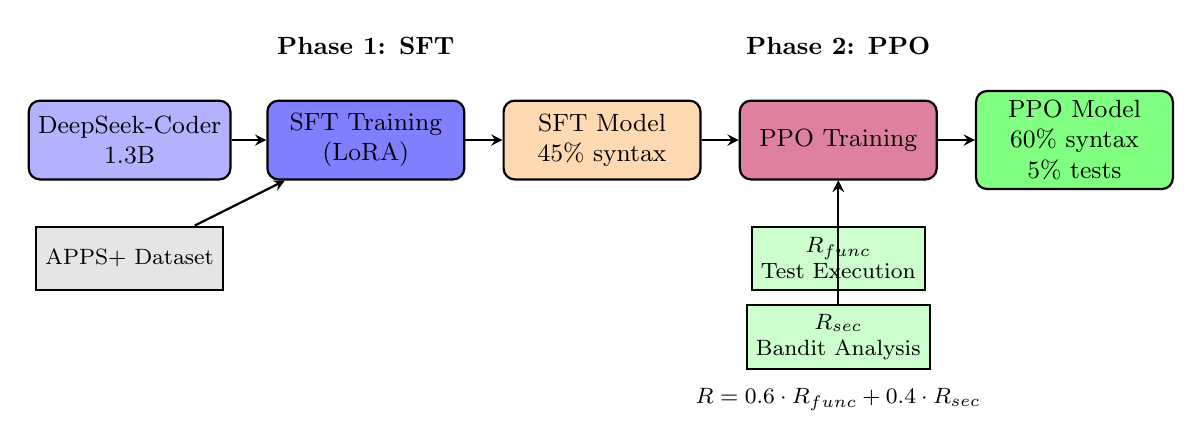
\begin{tikzpicture}[
    box/.style={rectangle, draw=black, thick, rounded corners, minimum width=2.5cm, minimum height=1cm, align=center, font=\small},
    data/.style={rectangle, draw=black, thick, fill=gray!20, minimum width=2cm, minimum height=0.8cm, align=center, font=\footnotesize},
    reward/.style={rectangle, draw=black, thick, fill=green!20, minimum width=2cm, minimum height=0.8cm, align=center, font=\footnotesize},
    arrow/.style={->, thick, >=stealth}
]

% Phase 1: SFT
\node[box, fill=blue!30] (base) at (0,0) {DeepSeek-Coder\\1.3B};
\node[data] (apps) at (0,-1.5) {APPS+ Dataset};
\node[box, fill=blue!50] (sft) at (3,0) {SFT Training\\(LoRA)};
\node[box, fill=orange!30] (sft_model) at (6,0) {SFT Model\\45\% syntax};

% Phase 2: PPO
\node[box, fill=purple!50] (ppo) at (9,0) {PPO Training};
\node[box, fill=green!50] (final) at (12,0) {PPO Model\\60\% syntax\\5\% tests};

% Reward components
\node[reward] (rfunc) at (9,-1.5) {$R_{func}$\\Test Execution};
\node[reward] (rsec) at (9,-2.5) {$R_{sec}$\\Bandit Analysis};

% Arrows
\draw[arrow] (base) -- (sft);
\draw[arrow] (apps) -- (sft);
\draw[arrow] (sft) -- (sft_model);
\draw[arrow] (sft_model) -- (ppo);
\draw[arrow] (ppo) -- (final);
\draw[arrow] (rfunc) -- (ppo);
\draw[arrow] (rsec) -- (ppo);

% Phase labels
\node[above of=sft, node distance=1.2cm, font=\small\bfseries] {Phase 1: SFT};
\node[above of=ppo, node distance=1.2cm, font=\small\bfseries] {Phase 2: PPO};

% Reward formula
\node[font=\footnotesize] at (9,-3.3) {$R = 0.6 \cdot R_{func} + 0.4 \cdot R_{sec}$};

\end{tikzpicture}
